1 pascal = $10^5$ bar = $7.50062 \cdot 10^{-2}$ torr

\section{Molmassen wichtiger Atome}

\renewcommand{\arraystretch}{1.3}
\begin{tabular}{c | c | c }
    \textbf{Symbol} & \textbf{Molekül}  & \textbf{Molmasse}                 \\
    \hline
    H               & Wasserstoff       & $1.008 \, \frac{\gram}{\mole}$    \\
    C               & Kohlenstoff       & $12.011 \, \frac{\gram}{\mole}$   \\
    N               & Stickstoff        & $14.007 \, \frac{\gram}{\mole}$   \\
    O               & Sauerstoff        & $15.999 \, \frac{\gram}{\mole}$   \\
    Al              & Aluminium         & $26.982 \, \frac{\gram}{\mole}$   \\
    Si              & Silicium          & $28.982 \, \frac{\gram}{\mole}$   \\
\end{tabular}\smallbreak

Elementi come $H_2$ sono e volte la molmassse di $H$
\renewcommand{\arraystretch}{1.3}

\section{Ansätze zu Aufgaben}

\subsection{Barometer}

\begin{minipage}[t]{0.38\columnwidth}
    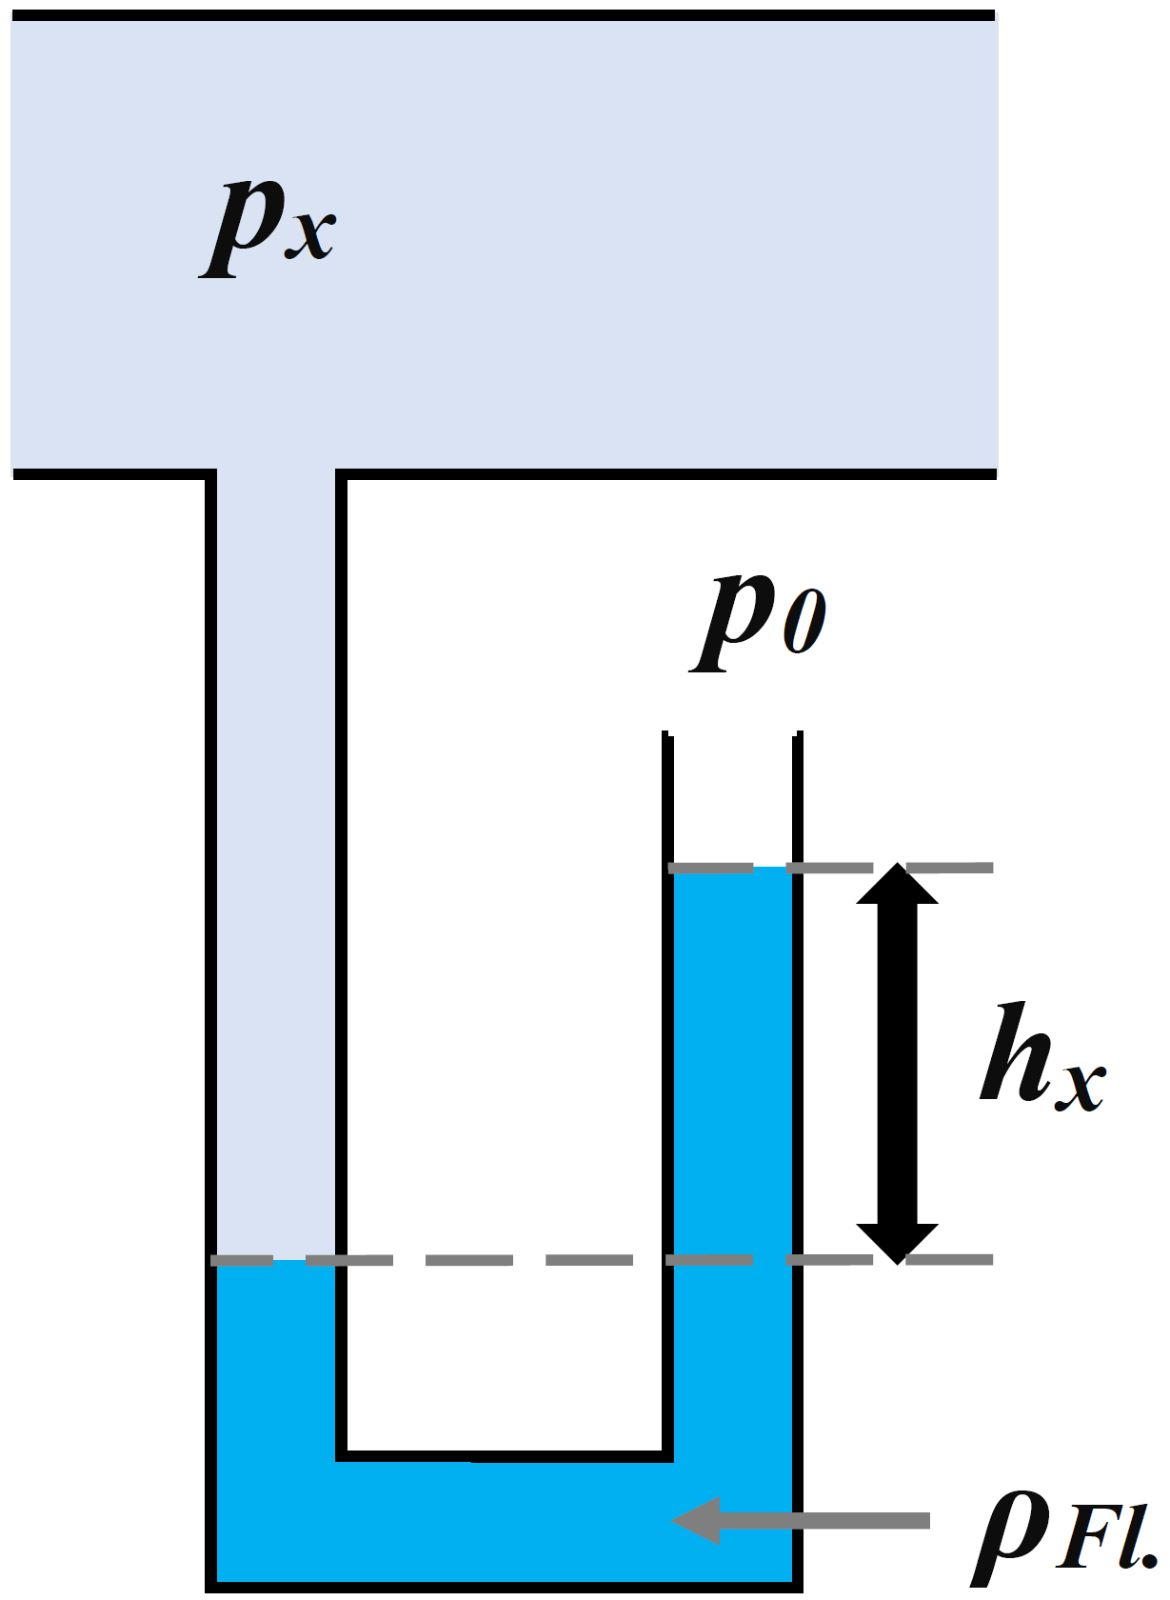
\includegraphics[width=\columnwidth, align=t]{images/manometer.jpg}
\end{minipage}
\hfill
\begin{minipage}[t]{0.5\columnwidth}
    $$ \boxed{ p_x = p_0 + \underbrace{ \rho_{Fl} \cdot g \cdot h}_{\substack{p_s}} } $$
 
    \begin{tabular}{ll}
        $p_x$   & Gemessener Druck  \\
        $p_0$   & Luftdruck         \\
        $p_s$   & Schweredruck (Dal fluido)
    \end{tabular}

    \medskip

    \textrightarrow\ Bernoulli \\
    \textrightarrow\ Kontinuität
\end{minipage}


\subsection{Tubo di Pitot (Tubo di Prandtl)}
Strumento per la misurazione della velocità di un fluido ($\rho_L$).

\begin{center}
    % Inserisci qui l'immagine
    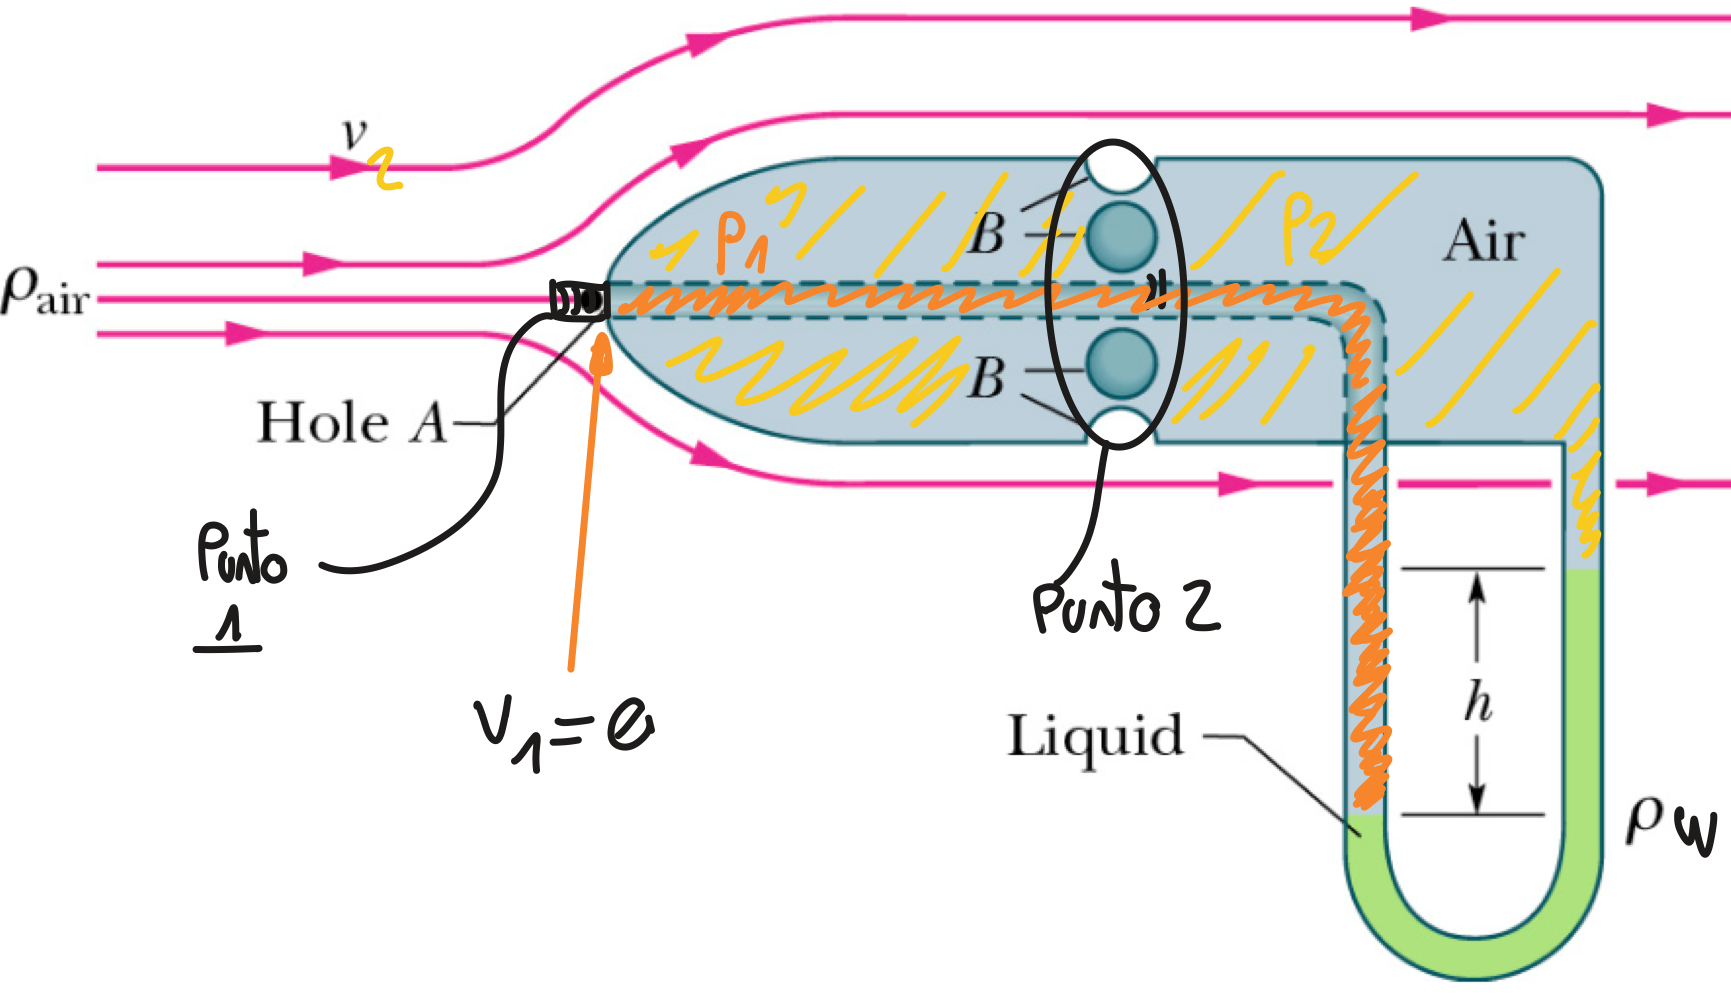
\includegraphics[width=0.73\columnwidth]{images/pitotrohr.png}
\end{center}

\textbf{Assunzioni:}
\begin{itemize}
    \item \textbf{Bernoulli orizzontale:} Poiché i fori $A$ e $B$ sono alla stessa quota 
    ($y_1 \approx y_2$), la differenza di pressione idrostatica dell'aria 
    ($\rho_L g \Delta y$) è trascurabile rispetto alla pressione dinamica.
    \item \textbf{Punto di ristagno (1):} In punta l'aria si ferma completamente $\Rightarrow v_1 = 0$.
    \item \textbf{Pressione statica (2):} Ai fori laterali l'aria scorre indisturbata $\Rightarrow v_2 = v$.
\end{itemize}

\vspace{0.3cm}
\textbf{Manometro a U:}
La differenza di pressione è bilanciata dal dislivello $h$ del liquido manometrico ($\rho_{Fl}$):
$$ p_1 = p_2 + \rho_{Fl} \cdot g \cdot h $$

\textbf{Equazione di Bernoulli:}
$$ p_1 + \frac{1}{2}\rho_L \cdot v_1^2 = p_2 + \frac{1}{2}\rho_L \cdot v_2^2 \qquad p_1 \text{ Sostituire con eq. manometro}$$ 
$$ p_2 + \rho_{Fl} \cdot g \cdot h = p_2 + \frac{1}{2}\rho_L \cdot v_2^2$$


\textbf{Soluzione finale:}
$$ \frac{1}{2} \rho_L v^2 = \rho_{Fl} \cdot g \cdot h \implies \boxed{v = \sqrt{\frac{2 \cdot \rho_{Fl} \cdot g \cdot h}{\rho_L}}} $$

\subsection{U-Rohr}

\begin{minipage}{0.35\columnwidth}
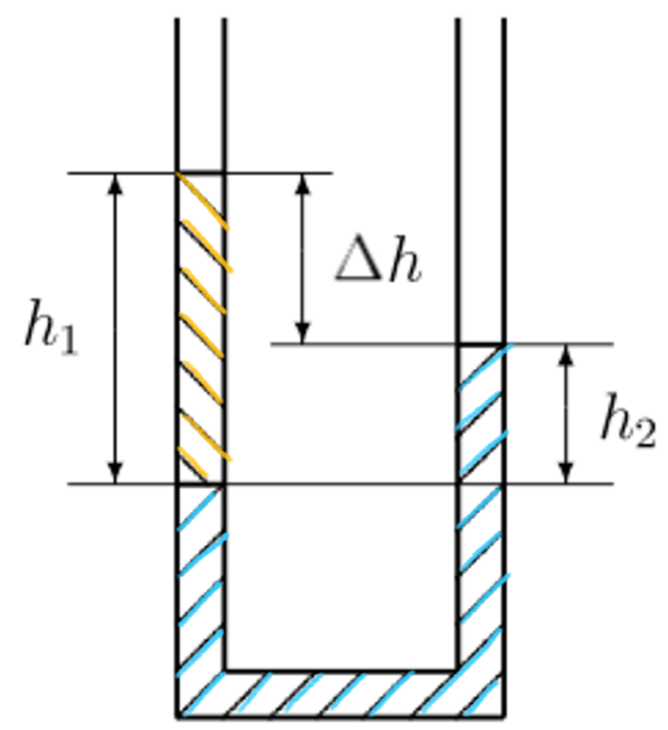
\includegraphics[width=\columnwidth, align=t]{images/u-rohr.png}
\end{minipage}
\hfill
\begin{minipage}{0.6\columnwidth}

    Ansatz: Druckgleichgewicht 

    $$ \boxed{ p_1 = p_2 } $$

    $$ \boxed{ \rho_1 \cdot h_1 = \rho_2 \cdot h_2 } $$
\end{minipage}

\subsection{Pumpe}

\vspace{-0.2cm}

$$ \boxed{ W = P \cdot t = F \cdot \Delta s = p \cdot A \cdot \Delta s = p \cdot \Delta V } \qquad  \qquad \boxed{ F = p \cdot A }  $$

$$ \boxed{ P =  \frac{W}{t} = \frac{p \cdot V}{t} = p  \cdot  \dot{V} } $$

\subsection{Torricelli}
\begin{minipage}{0.5\columnwidth}
    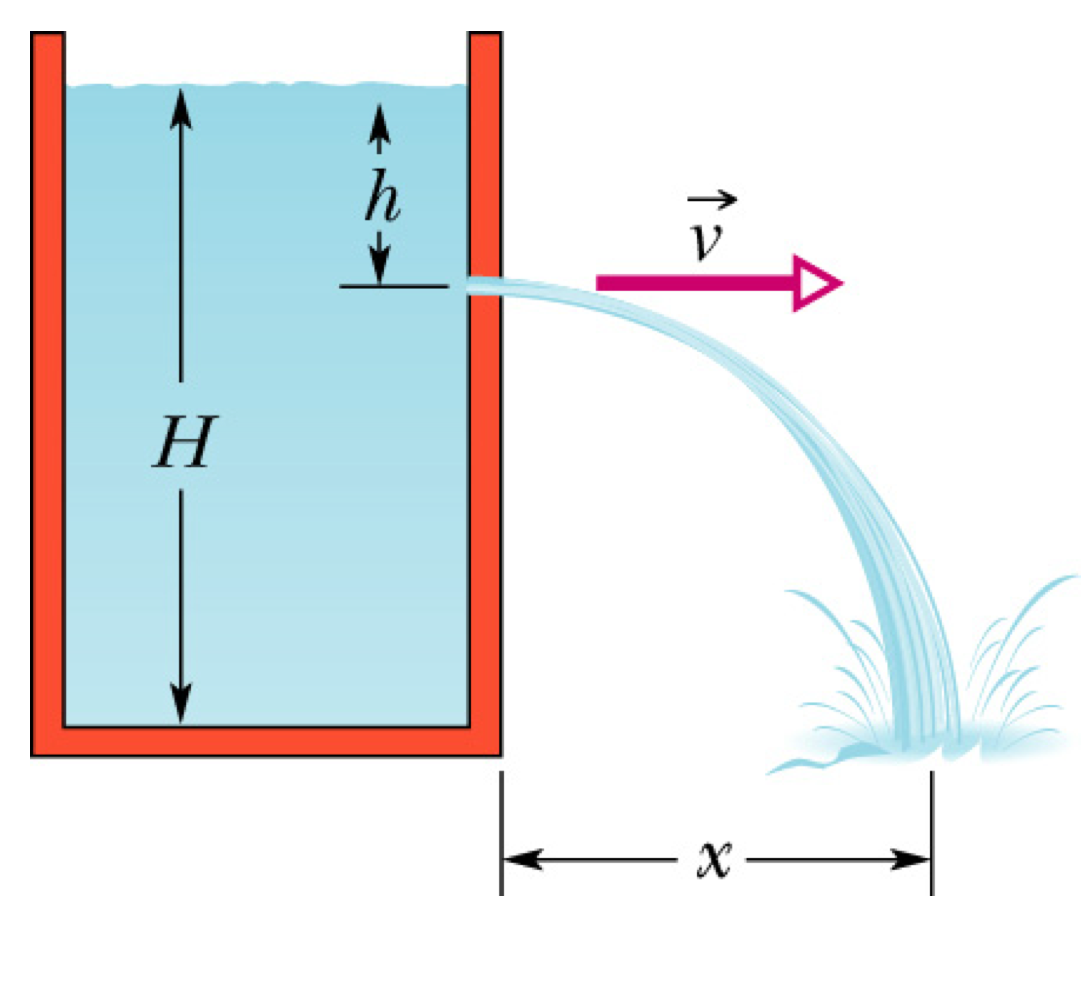
\includegraphics[width=\linewidth]{images/torricelli.png}
\end{minipage}
\begin{minipage}[b]{0.48\columnwidth}
    \cor{Attenzione} anche se il tubo andasse sopra 
    al livello dell'$\rm H_2O$ l'altezza viene sempre calcolata dal livello dell'acqua

    \[\boxed{v = \sqrt{2gh}} \qquad \boxed{x = 2\sqrt{h(H-h)}}\]
    
\end{minipage}  


\subsection{Bewegungen}

\vspace{-0.2cm}

\[\boxed{ P = F \cdot v } \qquad \boxed{F = \dot{m} \cdot \Delta v}\qquad \boxed{ E_{\rm kin} = \frac{1}{2} \, m \cdot v^2 } \]
\[\boxed{\dot{m} = \rho \dot{V}}\]



\subsection{Wasser mit Dampf erhitzen}

Ein Tasse mit $m_W = 200 \, \gram$ Wasser  mit einer Temperatur von $T_K = 20 \, \celsius$ wird an
der Wasserdampfdüse einer Kaffeemaschine mittels Wasserdampf erhitzt. \\
Der aus der Kaffeemaschine ausströmende Wasserdampf ist $T_H = 96 \, \celsius$ heiss. \\
Am Schluss haben Sie 10 \% mehr Wasser in der Tasse. (entspricht $m_D$)\\
Wie warm ist das Wasser nun?

$$ \text{Ansatz: 1. Hauptsatz} \quad \Delta Q_{\rm zu} = \Delta Q_{\rm ab} $$ 
$$ m_W \cdot c_W \, (T_M - T_K) = q_s \cdot m_D + m_D \cdot c_W \, (T_H - T_M) $$


\subsection{Eis in Wasser schmelzen}

In einem Gefäss beifinden sich $m_W = 1 \, \kilogram$ Wasser. \\
Dazu wird ein Eiswürfel von $m_E = 20 \, \gram$ gegeben. \\
Das Eis hat eine Temperatur von $T_E = -5 \, \celsius$ und das Wasser hat eine Temperatur $T_W$. Die Temperatur $T_0$ steht 
für $0 \, \celsius$ bzw. $275.15 \, \kelvin$ \\
Gesucht ist die Mischtemperatur $T_M$ 

$$ \Delta Q_{\rm ab} = \Delta Q_{\rm zu} $$
$$ m_W \cdot c_W \cdot (T_W - T_M) = m_E \cdot c_E \cdot (T_0 - T_E) + q_f \cdot m_E + m_E \cdot c_W \cdot (T_M - T_0) $$

\subsection[Concetto di temperatura Critica nelle bombole]
{Concetto di Temperatura Critica ($T_k$) nelle Bombole}

\begin{itemize}
    \item \textbf{Se $T_{amb} < T_k$ (es. $CO_2$ a $20^\circ C$):} 
    All'interno della bombola coesistono fase liquida e gassosa. La pressione indicata dal manometro è la \textit{pressione di vapore saturo} ($p_s$), che dipende solo dalla temperatura.
    \item \textbf{Comportamento:} Aprendo brevemente la valvola, la pressione rimane costante perché una parte del liquido evapora immediatamente per ripristinare l'equilibrio.
    \medskip
    \item \textbf{Se $T_{amb} > T_k$:} 
    La sostanza è esclusivamente allo stato gassoso (gas supercritico). Non può esistere liquido indipendentemente dalla pressione applicata.
    \item \textbf{Comportamento:} Aprendo la valvola, la pressione cala immediatamente poiché diminuisce la densità del gas senza che ci sia liquido a compensare la perdita di massa.
\end{itemize}\smallbreak

\section{Sistemi Termodinamici}
Un sistema termodinamico è un sistema fisico limitato spazialmente per il quale è possibile stabilire un bilancio energetico (e di massa, se aperto).

I sistemi si distinguono in base alla possibilità di scambiare materia o energia con l'ambiente circostante:

\begin{ctabular}{@{}lll@{}}
\toprule
\textbf{Sistema} & \textbf{Scambio di Materia} & \textbf{Scambio di Energia} \\ \midrule
\textbf{Aperto} & Consentito & Consentito (Lavoro e Calore) \\
\textbf{Chiuso} & Non consentito & Consentito (Lavoro e Calore) \\
\textbf{Isolato} & Non consentito & Non consentito \\ \bottomrule
\end{ctabular}

\subsection{Sotto-categorie e Casi Specifici}
\begin{itemize}
    \item \textbf{Sistema Adiabatico:} Non permette lo scambio di calore ($Q = 0$), ma permette lo scambio di lavoro ($W$). Esempio: compressione rapida.
    \item \textbf{Sistema Arbeitsdicht (Ermetico al lavoro):} Non permette lo scambio di lavoro meccanico.
    \item \textbf{Sistema Energiedicht (Ermetico all'energia):} Non permette alcuno scambio di energia (né calore né lavoro).
\end{itemize}

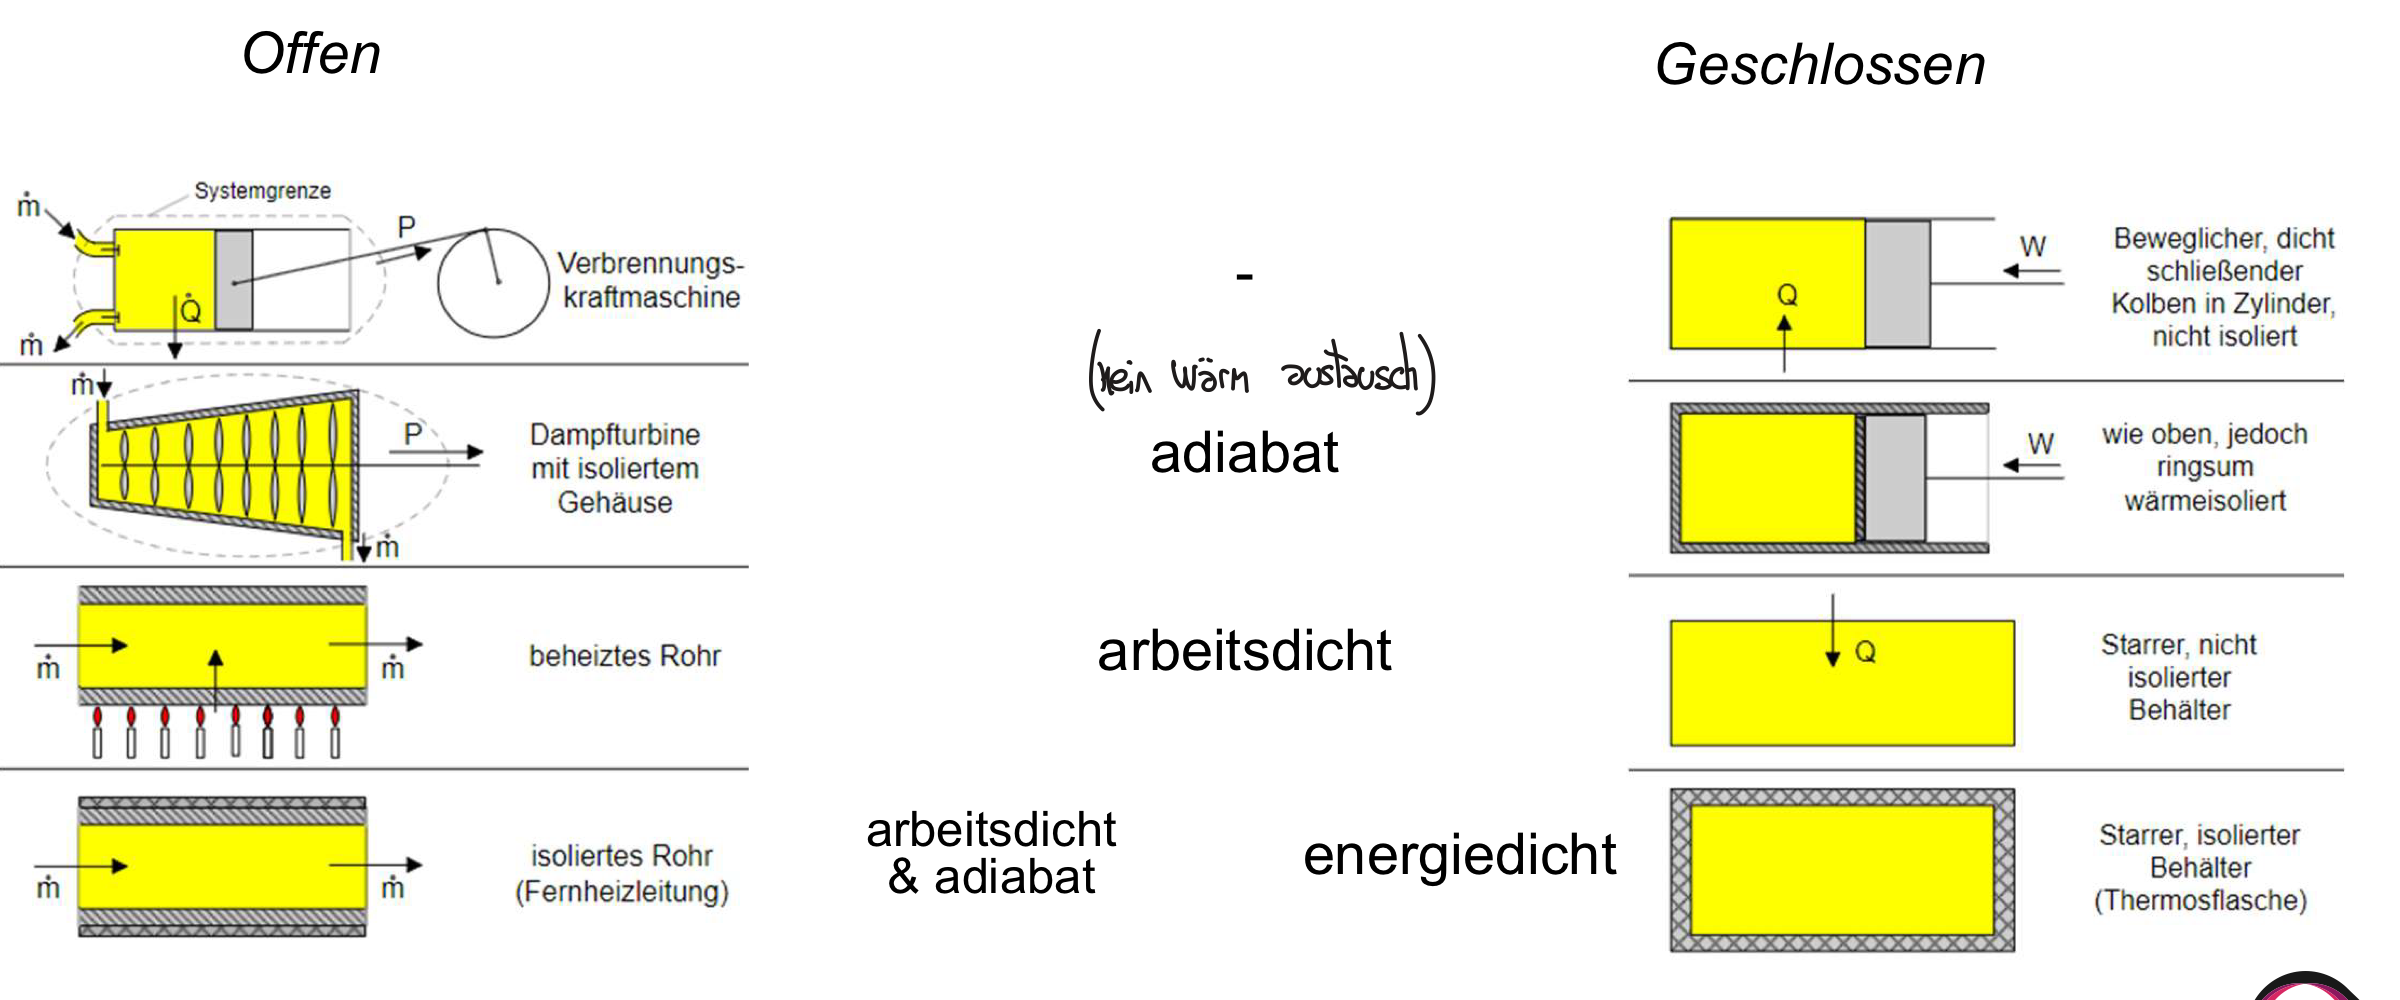
\includegraphics[width=\columnwidth]{images/thermodinamishce_systeme.png}

\section{Grandezze Termodinamiche}
\begin{itemize}
    \item \textbf{Grandezze di Stato:} Dipendono solo dallo stato attuale del sistema e non dal percorso seguito per raggiungerlo (es. Temperatura $T$, Pressione $p$, Volume $V$).
    \item \textbf{Grandezze di Processo:} Descrivono il modo in cui il sistema passa da uno stato all'altro (es. Calore $Q$, Lavoro $W$). Il loro valore dipende dalla velocità o dalla modalità del processo.
\end{itemize}